% ADS2 AE1 Report written in LaTeX by Inesh Bose

\documentclass{article}

%==============================================================================
%% Packages and Command Setting

\usepackage[utf8]{inputenc}
\setcounter{secnumdepth}{0}
\newcommand{\code}[1]{\texttt{#1}}
\usepackage{pgfplots}
\usepackage{geometry}
\usepackage{listings}
\usepackage[T1]{fontenc}
\usepackage{color}
\usepackage{float}
\usepackage{hyperref}
\usepackage[symbol]{footmisc}

\hypersetup{
    colorlinks,
    citecolor=black,
    filecolor=black,
    linkcolor=black,
    urlcolor=black
}
\renewcommand{\thefootnote}{\fnsymbol{footnote}}

\definecolor{mygreen}{rgb}{0,0.6,0}
\definecolor{mygray}{rgb}{0.5,0.5,0.5}
\definecolor{mymauve}{rgb}{0.58,0,0.82}

\lstset{ %
  backgroundcolor=\color{white},   % choose the background color
  basicstyle=\footnotesize,        % size of fonts used for the code
  breaklines=true,                 % automatic line breaking only at whitespace
  captionpos=b,                    % sets the caption-position to bottom
  commentstyle=\color{mygreen},    % comment style
  escapeinside={\%*}{*)},          % if you want to add LaTeX within your code
  keywordstyle=\color{blue},       % keyword style
  stringstyle=\color{mymauve},     % string literal style
}


%==============================================================================
%% Title Page

\title{Algorithms and Data Structures \\ Assessed Exercise 2}
\author{Inesh Bose}
\date{}

\begin{document}

\maketitle
\vspace{2cm}
\tableofcontents
\addtocontents{toc}{\protect\thispagestyle{empty}}
\pagenumbering{gobble}

%==============================================================================
%% Part 1 : Page 1

\newpage

\section{Part 1}
The Dynamic Set ADT has been implemented in Java using \textbf{parameterised} Doubly Linked List and Binary Search Tree in \code{DoublyLinkedList.java} and \code{BinarySearchTree.java} respectively. Both of them have methods \code{add(Item x), remove(Item x), isEmpty(), isElement(Item x), size(), union(), intersection(), difference() and subset()}. \\

\bigskip

\subsection{Doubly Linked List}
A doubly linked list is similar to a linked list, but each node has an additional \code{prev} attribute. While it helps making some operations simpler and more efficient, it can lead it to memory overhead. \\
\begin{lstlisting}[language=Java]
        public class DoublyLinkedList<Item>{
            private Node<Item> head, tail;
            private int size;
            private static class Node<Item>{
                private Item key;
                private Node<Item> next, prev;
            }
        ....
\end{lstlisting}

\bigskip

\subsection{Binary Search Tree}
Binary Search Tree has nodes / leaves, each pointing to two other nodes / leaves \\(depending upon the value of key) which could be the root of another subtree. \\
\begin{lstlisting}[language=Java]
        public class BinarySearchTree<Item> {
            private Node<Item> root;
            private static class Node<Item>{
                private Item key;
                private Node<Item> left, right, p;
                private int size;
            }
        ....
\end{lstlisting}

\bigskip

\subsection{ADTRunner.java}
This file contains the main method that displays the running time for each file / dataset for both implementations of the ADT. It also includes commented-out lines in order to view the ADT.
\begin{lstlisting}[language=Java]
        // String path = "M:/ADS/Files/";  /** Change Path Here */
        /** If this gives "(Access denied)" or some error,
        comment the line below and use hardcoded path above. */
        String path = System.getProperty("user.dir")+"/Files/";
\end{lstlisting}

%==============================================================================
%% Part 1 : Page 2 (Graph)

\newpage
\newgeometry{top=2in,bottom=0.8in}

\subsection{Running Times}
The following is the graph indicating the running time for each operation in both implementations.\\ The computer was a Dell XPS 15 with Intel Core i7-9750H (2.60GHz) and 16GB DDR4 RAM.\\
The file used was \code{int20k.txt} and time was measured in nanoseconds.

\bigskip

\pgfplotsset{width=15cm,compat=1.9}
\begin{center}
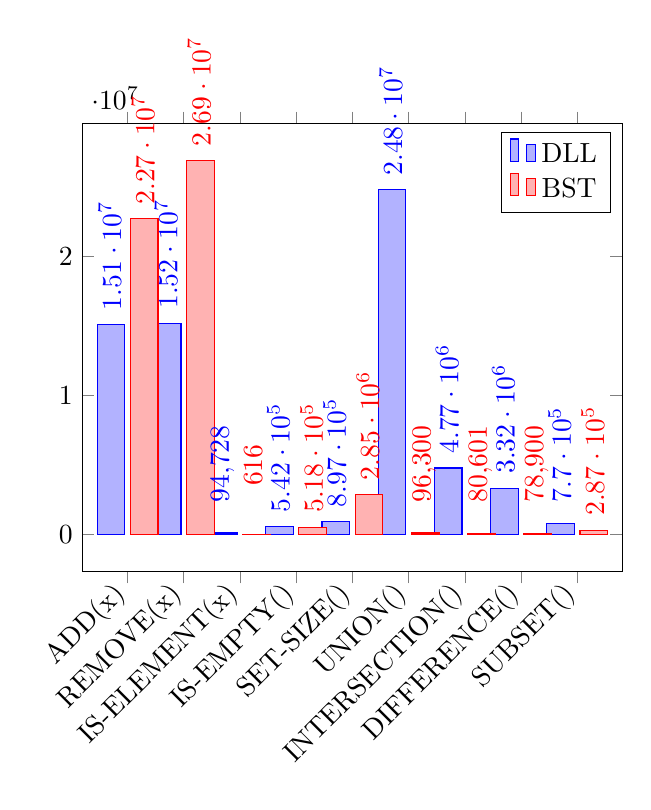
\begin{tikzpicture}
\begin{axis}[
    ybar,
    nodes near coords,
    every node near coord/.append style={rotate=90,anchor=north,yshift=8pt,xshift=25pt},
    enlargelimits,
    symbolic x coords={ADD(x), REMOVE(x), IS-ELEMENT(x), IS-EMPTY(), SET-SIZE(), UNION(), INTERSECTION(), DIFFERENCE(), SUBSET()},
    xtick=data,
    x tick label style={rotate=45,anchor=east},]
    \addplot coordinates {
        (ADD(x), 15083013)
        (REMOVE(x), 15206958)
        (IS-ELEMENT(x), 94728)
        (IS-EMPTY(), 541700)
        (SET-SIZE(), 896600)
        (UNION(), 24795901)
        (INTERSECTION(), 4773735)
        (DIFFERENCE(), 3321800)
        (SUBSET(), 770400)
    };
    \addplot coordinates {
        (ADD(x), 22709601)
        (REMOVE(x), 26899600)
        (IS-ELEMENT(x), 616)
        (IS-EMPTY(), 518399)
        (SET-SIZE(), 2853801)
        (UNION(), 96300)
        (INTERSECTION(), 80601)
        (DIFFERENCE(), 78900)
        (SUBSET(), 287201)
    };
\legend{DLL, BST}
\end{axis}
\end{tikzpicture}

\small{Note: The running times of ADD(x) for DoublyLinkedList is 100x more than what is displayed.\\ This was done to maintain the Y axis range.}

\end{center}

\restoregeometry

%==============================================================================
%% Part 1 : Page 3 & Part 2

\newpage

\subsection{Complexity of \code{add(x)} and \code{isElement(x)}}
The implications of maintaining the doubly linked list sorted on the complexity of \code{add(x)} and \code{isElement(x)} is that adding a node would cause the complexity of \code{add(x)} to be O($n$); the same would be the case for \code{isElement(x)} changing the complexity of O($n$) causing the entire complexity to go from O($n logn$) to O($n1+n2$).

\bigskip

\subsection{UNION(S,T)}
A possible, better, implementation is to convert the BST into a sorted list causing the complexity to be O($n$), then merging the two converted BSTs into \textbf{one} sorted list, making the complexity to be O($n1+n2$) and finally creating a new Binary Search Tree with elements from the list making the complexity O($n$). Therefore, the final complexity would be O($n1+n2$).


\section{Part 2}

\bigskip

\subsection{Empirical Study}
The two implementations of the Dynamic Set ADT were populated with elements from the dataset \code{int20k.txt} and then 100 random numbers were generated in the interval [0, 49999] and then \code{isElement(x)} was called. The following is the result:

\smallskip

\begin{table}[H]
\centering
\begin{tabular}{|l|l|l|}
\hline
            & DLL    & BST \\ \hline
 Time (ns)  & 94,728 & 616 \\ \hline
\end{tabular}
\end{table}

\smallskip

An explanation for this result is that Binary Search Trees satisfy \textit{binary-search-tree property} which helps for searching therefore being much more efficient. This also causes the complexity of a Binary Search Tree to be half of Doubly Linked List which is O($n$).

\bigskip

\subsection{SET-SIZE(S)}
The \code{size()} method for the two implementations returns the size of the ADT (\code{int}). The implementation of Doubly Linked List maintains the size in \code{int size} which is incremented and decremented when an element is added and removed respectively. This value is simply returned when \code{size()} is called. Binary Search Trees, however, have subtrees, therefore each node has \code{int size} and \code{size()} calls a recursive function that adds the value for each node and then return it. \\
The size for both implementation of the ADT having data from \code{int20k.txt} is 16,536.

\bigskip

\subsection{Height of the BST}
The \code{height()} method in \code{BinarySearchTree.java} is a recursive function that returns the height of a tree by splitting the tree is two subtrees. \\
The output for a Binary Search Tree containing the data from \code{int20k.txt} is 35.

\end{document}